\chapter{Methods}

\section{Classical Computer Vision-based Approach}

This section is related to all the experiments done on the classical computer 
vision-based approach. The general scheme of the driver's attention model is 
shown in Figure \ref{fig:driver_attention}. 
The model is divided into four main stages: data synchronization, homography 
projection of the gaze, scene perception, and the driver's behavioral model. 

The data synchronization stage is responsible for aligning the data from the 
different sensors. In particular it is important that gaze data and 
images from the 
eye-tracking glasses are well synchronized each other and with video frames 
from the camera installed on the roof top of the car.

The homography projection of the gaze stage is responsible for projecting the 
gaze of the driver from the ETG camera plane to the roof top camera plane.
In this way we have a wider, more stable and accurate representation of 
the outside environment.
It is possible to 
estimate the homography transformation making the approximation that the matched 
keypoints are far away enough from the vehicle. This is a reasonable 
approximation since the driver is usually looking at the road and the objects 
far away from the vehicle. Moreover, the baseline of the stereo vision system is 
small compared to the depth of the keypoints.
The optimal way to estimate the projection would be through the epipolar 
geometry, estimating the fundamental matrix and the essential matrix. 
However, we have an uncalibrated stereo setup, and the baseline between the two 
cameras is not fixed. Even though it could be possible to integrate GPS data 
to estimate the two matrices, there is a consistent noise error that affects 
accuracy of the estimation.
The homography estimation is then divided in three steps: detection of keypoints 
in the two images through the SIFT algorithm, matching of the keypoints through 
RANSAC, and estimation of the homography matrix through the least squares method.

The scene perception stage is responsible for detecting and tracking the vulnerable 
users in the scene, such as pedestrians and cyclists. The detection is done 
through the YOLOv8 algorithm and the tracking through ByteTrack. In this way 
it is possible to compare the gaze of the driver with the state of the targets, 
including their position.

Finally, on the top, there is the driver's attention model. The responsibility 
of this block is to classify dangerous scenarios given the data from the 
driver and the scene. However, this block is sensitive to the quality of the 
signals of the previous stages.

\begin{figure}
    \centering
    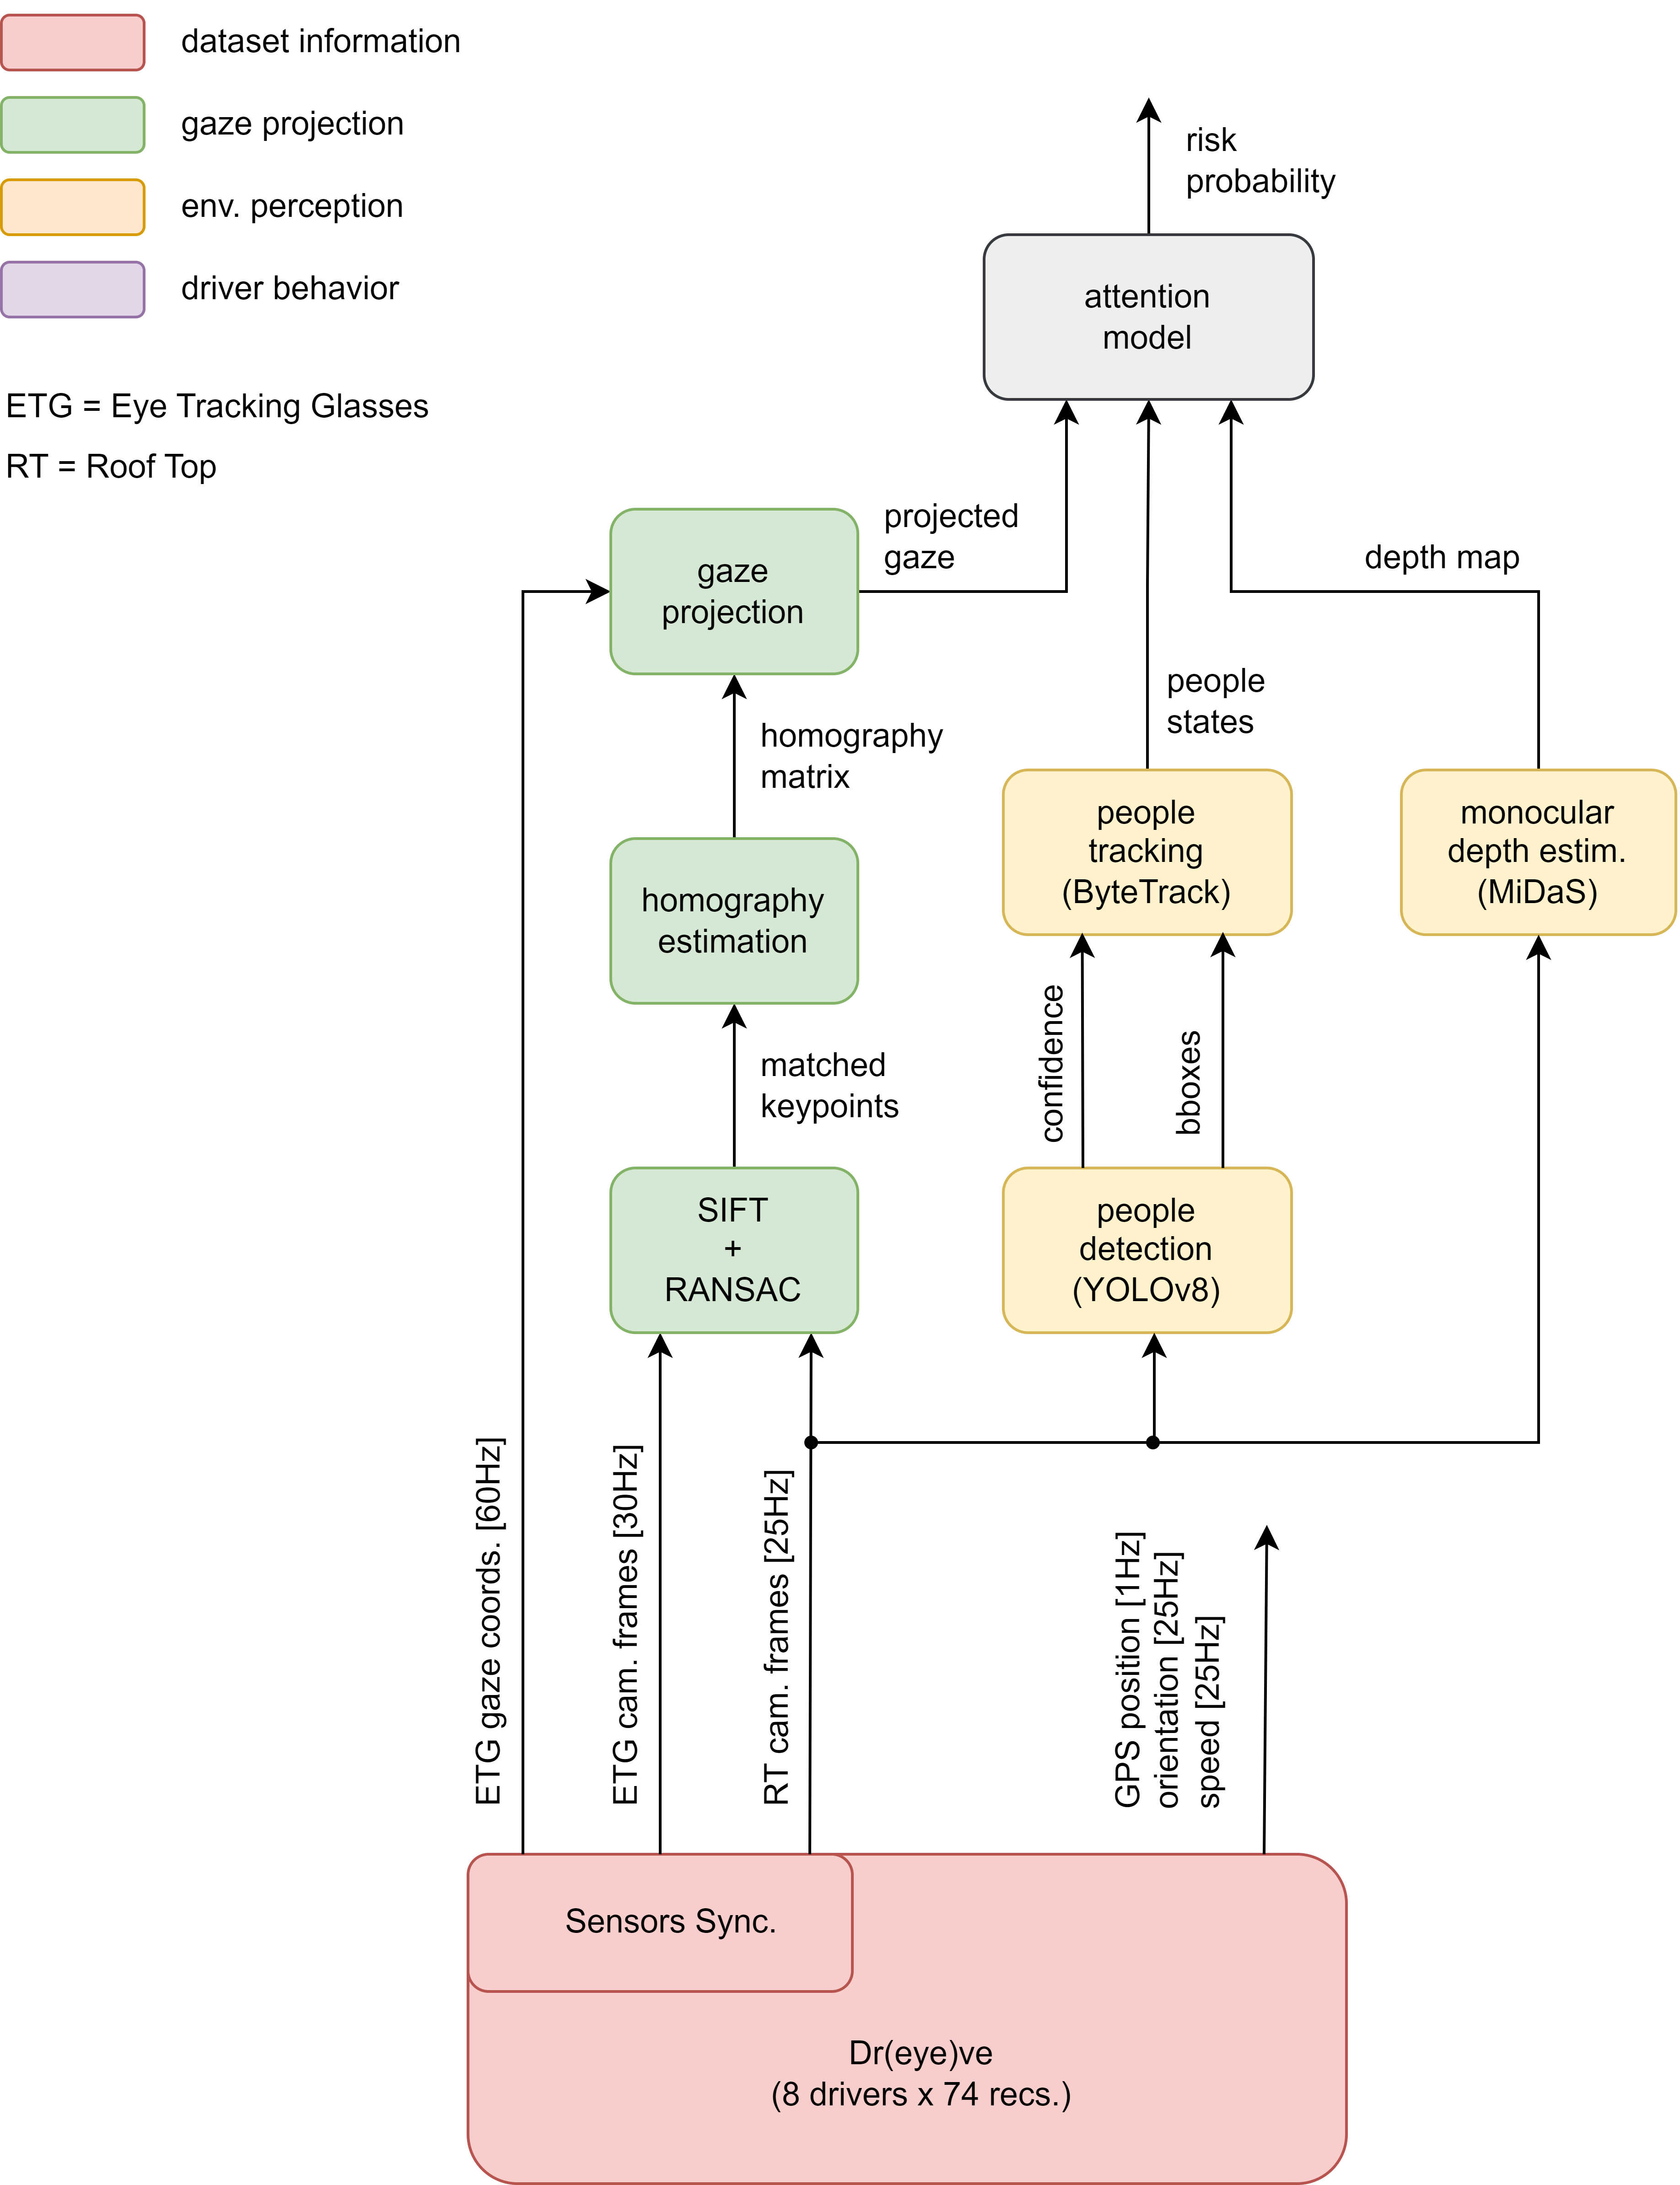
\includegraphics[width=0.9\textwidth]{images/dreyeve/classic_scheme.png}
    \vspace*{0.6cm}
    \caption{The overall driver's attention scheme. It is divided into four main 
    stages: data synchronization, homography projection of the gaze, scene 
    perception and the driver's behavioral model.
    }
    \label{fig:driver_attention}
\end{figure}

\subsection{Homography Data Structure}
The Dr(eye)ve dataset is composed of 74 sequences of five minutes each. 
Moreover, the two cameras are not synchronized. 
The ETG camera has a frame rate of 30 fps, while the roof top camera has a 
frame rate of 25 fps. It is also important to notice that there are some videos 
that was recorded at slightly different frame rates. All the synchronization data 
are provided in the dataset.

Therefore, we decided to implement 
an interface to preprocess all the frames and synchronize them.
After the synchronization, we compute all the homographies and store them in a 
file. This file is then used to project the gaze of the driver in the roof top 
camera plane.
Furthermore, we chose to store other informations related to the quality of the 
estimation.
The data structure is described in Figure \ref{fig:homography_data_structure}:
it is a list of lists where each element is a unique sample that has the 
following fields: the gaze coordinates in the ETG and RT camera planes, the 
homography matrix, detected keypoints on the two planes, and the number of 
matchings between them.

\begin{figure}
    \centering
    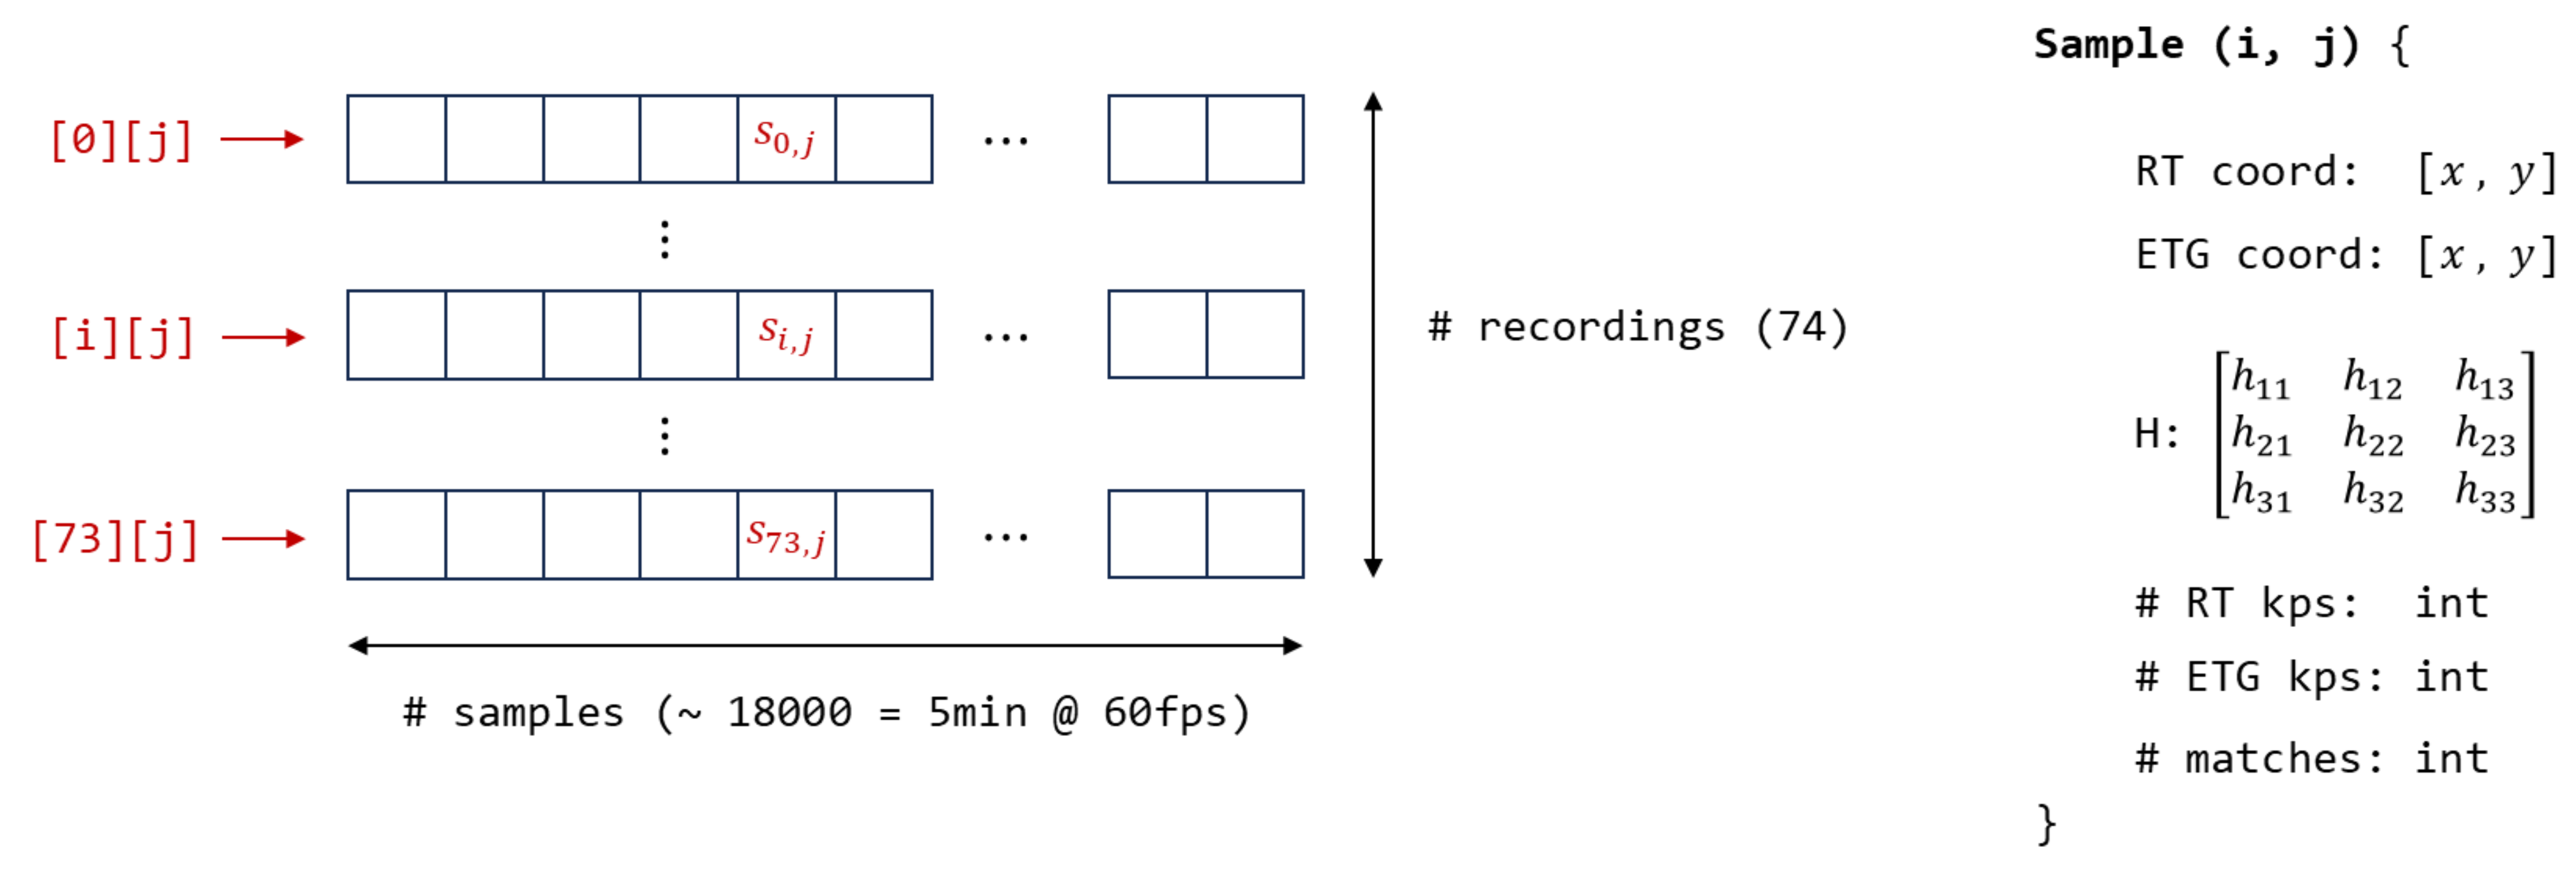
\includegraphics[width=\textwidth]{images/dreyeve/homography_data.png}
    \caption{The data structure used to store the homographies.
    \textbf{Left}: Each element is a specific sample in the i-th video, at 
    the j-th frame.
    \textbf{Right}: The attributes of each sample.}
    \label{fig:homography_data_structure}
\end{figure}

\subsection{Stereo Camera System Setup}
The cameras recording system can be reconducted to an uncalibrated stereo vision 
setup. In particular, the two cameras are not aligned and the baseline is not 
fixed. However, this is a problem for the projection of 3D world points between 
the two cameras. In fact, homography is a planar transformation, 
and it is possible to estimate the projection matrix if keypoints lie on the 
same plane.
For this reason we decided to make the approximation that the 
keypoints are far away enough from the vehicle. This is a reasonable 
approximation since the driver is usually looking at the road and the objects 
far away from the vehicle. Moreover, the baseline of the stereo vision system is 
small compared to the average depth of the keypoints.

In this way, it is not necessary to know intrinsic and extrinsic parameters of 
the cameras, such as focal length, resolution, and distortion coefficients. 
This approach is also proposed in the Dr(eye)ve paper \cite{dreyeve}.


\subsection{Targets Data Structure}
From the Dr(eye)ve dataset, we extracted the bounding boxes of the vulnerable 
road users, such as pedestrians and cyclists.
Moreover, through ByteTrack \cite{bytetrack}, we tracked the targets to have a 
spatio-temporal representation of the scene. Then, we compare the projected gaze 
of the driver with the location of targets. 

However, it is necessary to consider the quality of the tracking. Even though 
ByteTrack was specifically designed to track also overlapping objects, in driving 
scenarios it is not uncommon to have tracking failures. To partially mitigate 
the problem, we set two different states for each target: a 
\emph{detection} state and an \emph{observation} state.
\begin{itemize}
    \addtolength\itemsep{-2mm}
    \item \textbf{Detection}: the target is being detected and tracked by the algorithms.
    \item \textbf{Observation}: the target is being observed by the driver.
\end{itemize}

\begin{figure}
\centering
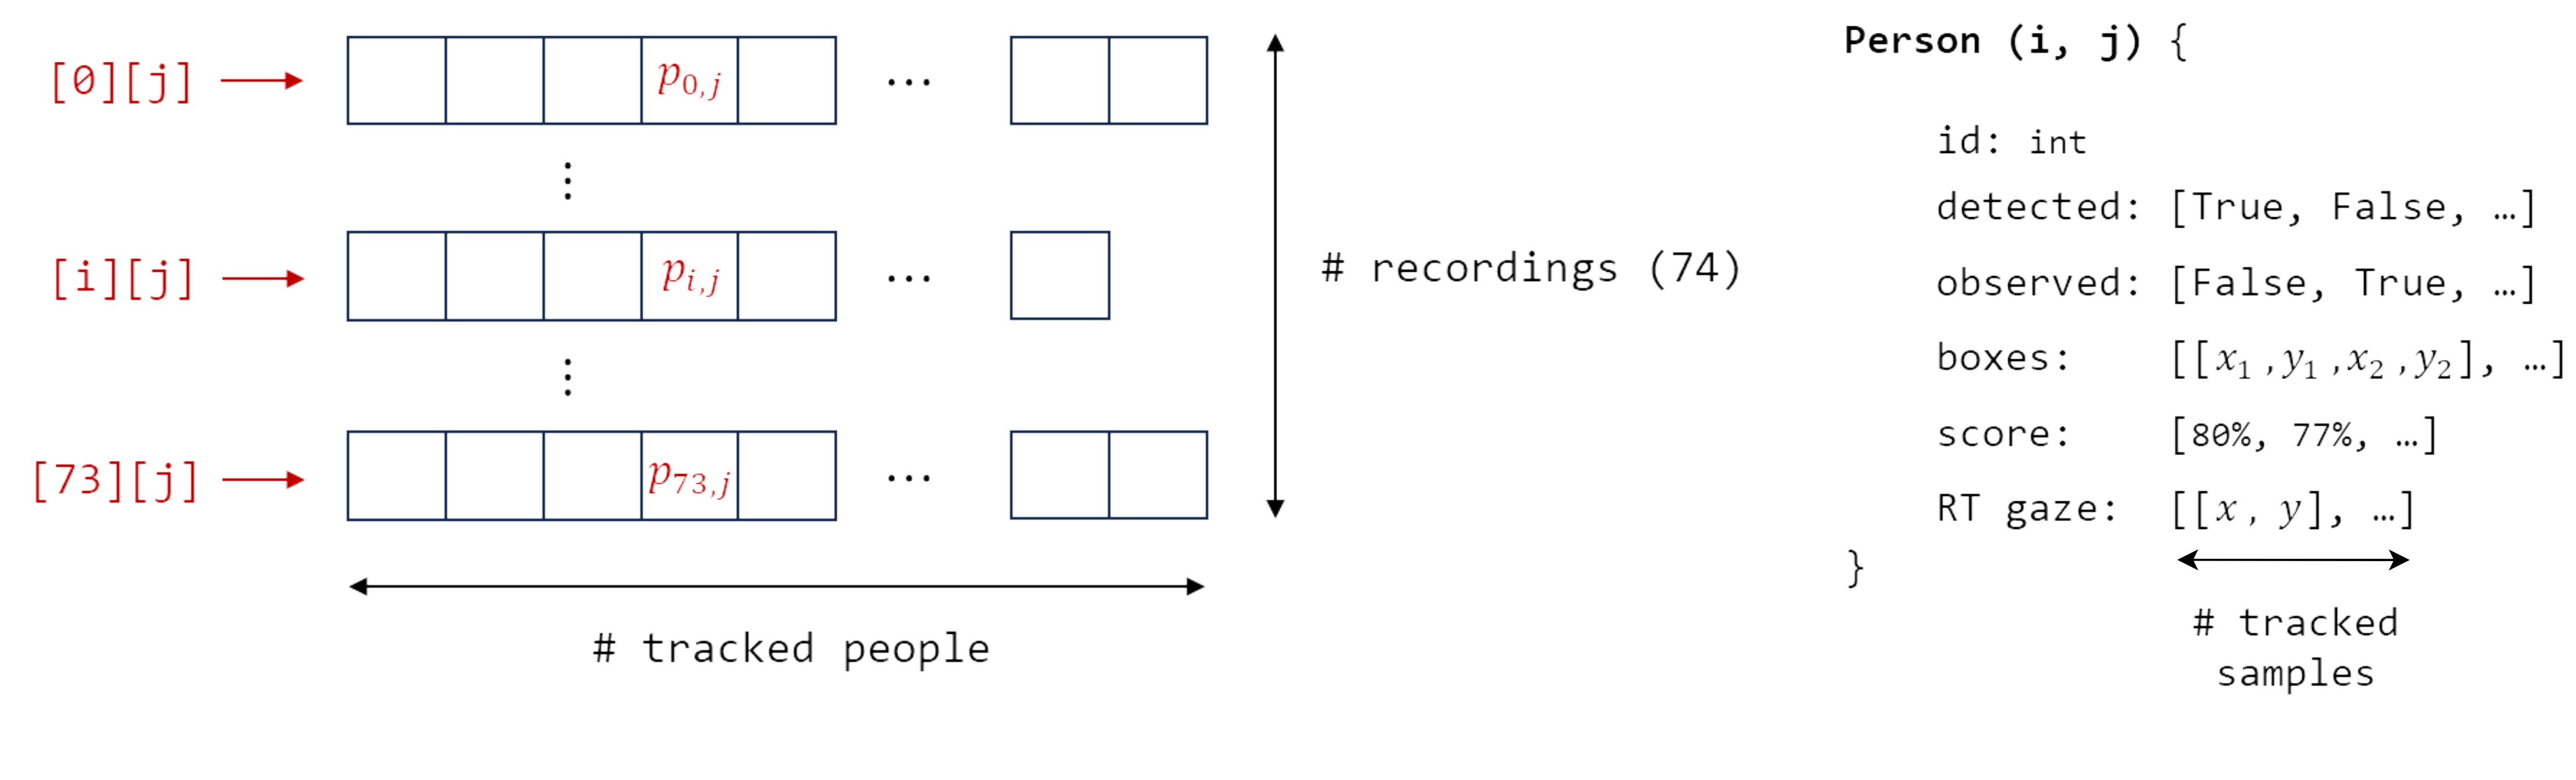
\includegraphics[width=\textwidth]{images/dreyeve/targets_data.png}
\caption{The data structure used to store targets' states.
\textbf{Left}: Each element is a specific person, which contains the set of 
states during all its tracking.
\textbf{Right}: The attributes of the tracked person during time.
}
\label{fig:targets_data_structure}
\end{figure}
Through this approach, we can make sure if a person is both detected by the 
algorithm and observed by the driver. Without storing the detection data, there 
can be some unclear situations where the driver is looking at a target that is 
partially or completely occluded. That can happen because ByteTrack keeps the 
tracking of occluded targets through a Kalman filter. 
The data structure is represented in details 
in Figure \ref{fig:targets_data_structure}: it is a list of lists where each 
element is a unique person that has been tracked in the respective video.

Each person has the following list of states: a unique tracking ID, the 
detection states, the observation states, the bounding boxes' coordinates with 
the confidence score, and the coordinates of the projected driver's gaze.

\subsection{Adding Depth Information}
Targets' depth information can be very informative for the driver's attention 
model. In fact, the driver is usually more interested in the objects that are 
closer to the vehicle.
Considering the cameras' setup there are three main ways to include depth 
information of the scene: using a neural network to estimate the depth of the 
detected objects from the bounding box dimensions, leveraging the stereo vision 
data and car's location information (GPS and speed) to estimate the depth of 
similar keypoints in consecutive timeframes, or to compute a monocular depth 
map through a pretrained model.

The first approach is the simplest and the fastest, but it is also the less 
accurate. In fact the depth of an object is not only related to its dimensions, 
especially for people. Bounding boxes can vary depending on the target age, pose, 
occlusions and if they are riding a vehicle, like a bicycle. 
Moreover, a custom calibration should be made at least for each camera model, 
with its dedicated lens and image sensor. Image distortion could heavily affect 
the quality of predictions. However, this is not feasible in our case because 
we do not have any ground truth information to fine-tune the model.
Some recent works on targets' depth estimation with stereo vision systems were 
proposed in \cite{li2019stereo}, \cite{Peng_2020_CVPR}. There are also studies 
on retrieving the depth of objects from monocular images \cite{bbox_mde}.

The second approach is the most accurate and robust, but it requires an accurate 
calibration of the stereo vision system to perform well. Moreover, data depth 
is only related to correspondent keypoints. This means that if no matching 
keypoints related to a target are found, it is not possible to estimate its 
depth. Finally, the stereo vision system is not always reliable, especially when 
it is uncalibrated and the baseline is not fixed and relatively small compared to 
the average depth of the keypoints. The roof top camera has a wide field of 
view because it uses a wide angle lens, and then an anti-distortion algorithm 
is computed. This affects the quality of the depth estimation.
Recently some self-calibration methods have been proposed 
\cite{sfm_self_calibration1}, \cite{sfm_self_calibration2}, but they are not

The third approach is the most versatile and suitable to the specific application.
In fact, the dense depth map computed by the pretrained model is not related to the 
ETG camera and allows to estimate the depth of all the objects in the scene.
The model is trained on a large dataset and is able to generalize well to 
different scenarios. The only drawback is that the depth map is not absolute. 
This means that it is not possible to estimate the distance of objects in meters, 
but through a relative scale depending on the maximum and minimum depths of the 
scene. However, this should not be able to compromise the quality of the 
driver's attention model because that is the same approach we use as humans 
when driving. However, we actually compute a hybrid approach where we use a sort 
of stereo vision system through our eyes and our knowledge and past experience 
to make an approximate estimation of the depth of the objects.
In the experiments section we will show the performance of pretrained MiDaS 
\cite{midas}.

\begin{figure}
\centering
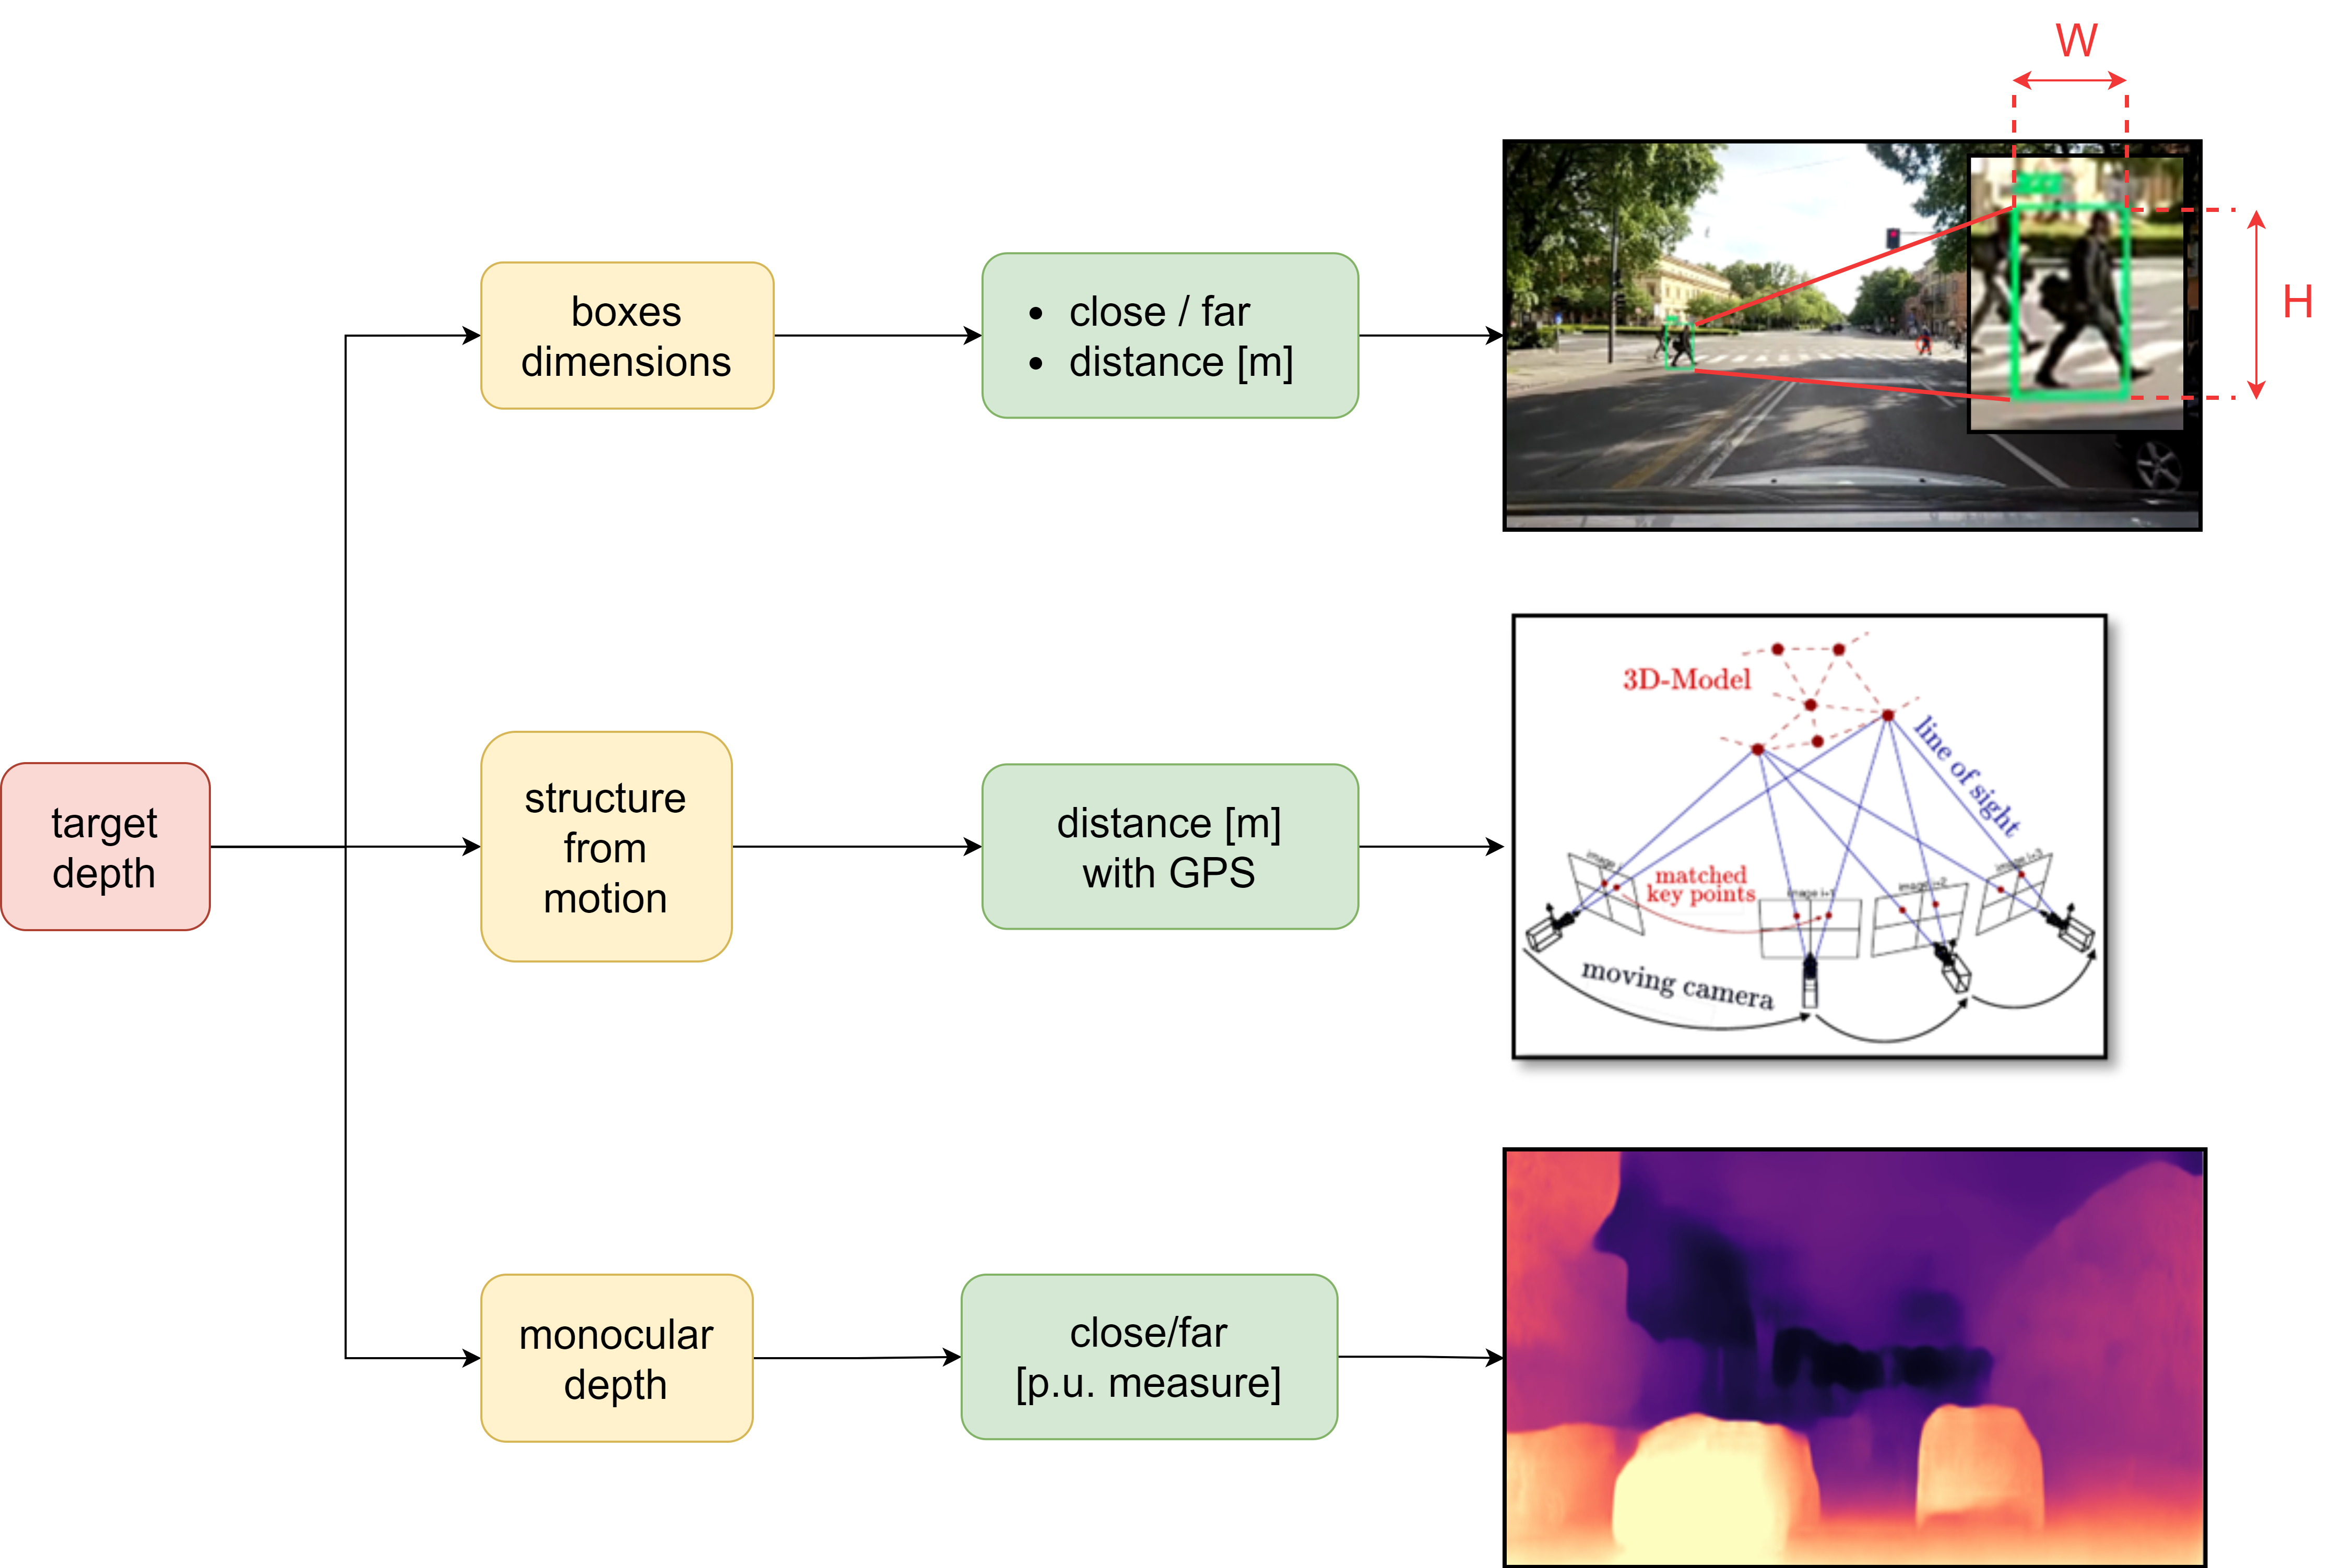
\includegraphics[width=\textwidth]{images/dreyeve/depth_estimation.png}
\caption{Summary of the possible three methods to estimate the depth of targets.}
\label{fig:depth_estimation}
\end{figure}



\subsection{Adding Spatial Information}
Spatial
\begin{figure}
\centering
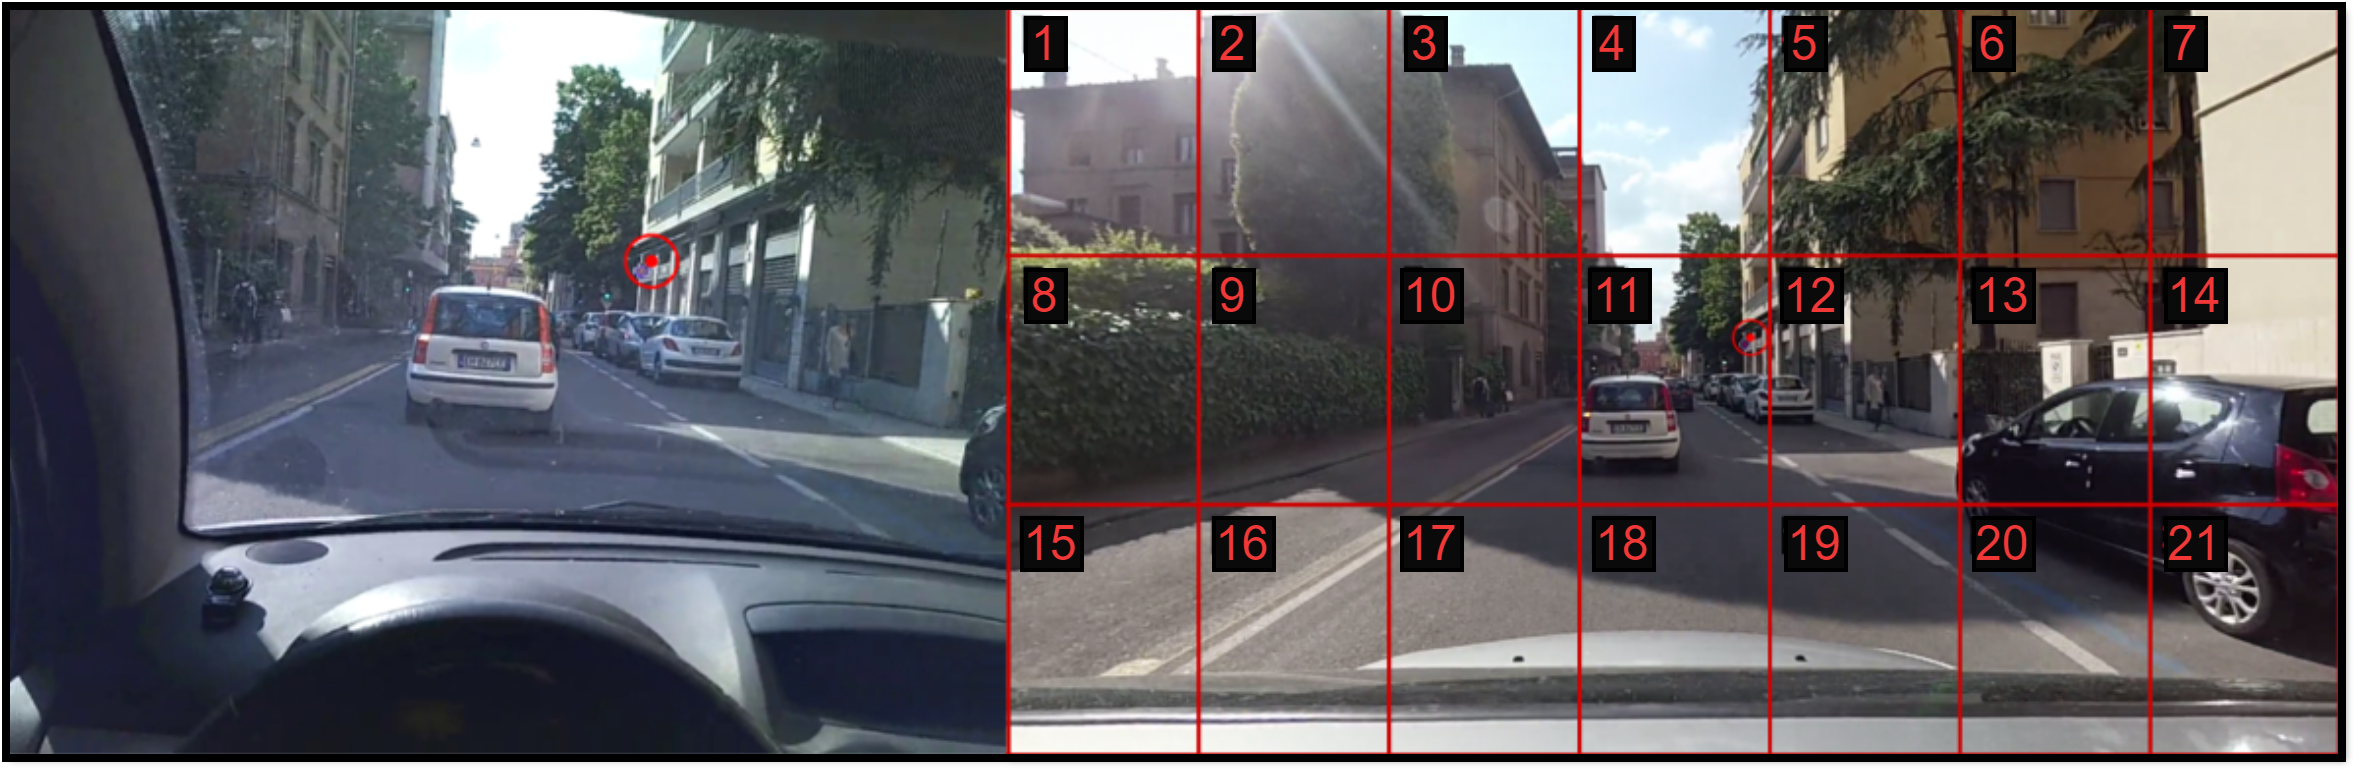
\includegraphics[width=\textwidth]{images/dreyeve/rt_cam_grid.png}
\caption{Division of the roof top camera view in a 3x7 grid.}
\label{fig:rt_camera_grid}
\end{figure}


\section{Deep Learning-based Approach}

\subsection{Attention Map for Anomaly Detection}

\subsection{The Artificial Bias}

\subsection{Data Preprocessing of Dr(eye)ve}

\subsection{Data Preprocessing of BDD100k}


\subsection{Handling Unbalanced Data}

\subsubsection{Evaluation Metrics}

\subsubsection{Data Augmentation}

% \subsubsection{Upsampling}

% \subsubsection{Downsampling}	

\subsubsection{Weighting Loss Function}

% \subsubsection{Synthetic Minority Oversampling Technique (SMOTE)}

% \subsection{Receiver Operating Characteristic (ROC) Curve}